\chapter{The branching fractions of \BsDsK~and \BdDsK}
\label{chp:DsK_BF}

% Get the page number of Fig. 1 in the paper
\newcount\DsKBFFigPage
\DsKBFFigPage=\thepage
\advance\DsKBFFigPage by 3

\lettrine{T}{he}~branching fractions of the decays \BsDsK~and \BdDsK~are interesting for several reasons.
First of all, the process \BsDsK~is a benchmark for decay-time-dependent measurements of \CP~violation in tree decays, and a dedicated analysis of its branching fraction and its backgrounds aid such a measurement.
Furthermore, the branching fraction of the process~\BsDsK can be related to its counterpart~\BsDsPi using the known differences in CKM~factors, decay constants, and kinematic properties.
However, this ratio has been found to be in tension with the theoretical expectations~\cite{DeBruyn:2012jp}.
The decay~\BdDsK, in turn, is interesting since it occurs, to first order, only through the suppressed exchange topology (see Fig.~1 on Page~\the\DsKBFFigPage).
Therefore, a measurement of its branching fraction can yield information on exchange topologies in general.
The measurement of these branching fractions is published in \mbox{JHEP} under the title ``Determination of the branching fractions of \BsDsK and \mbox{\BdDsK''}~\cite{LHCb-PAPER-2014-064}\footnote{
    Author of this thesis is corresponding author of the publication, and main contributor to the analysis.}
, which is reproduced here as \cref{chp:DsK_BF} of this thesis.

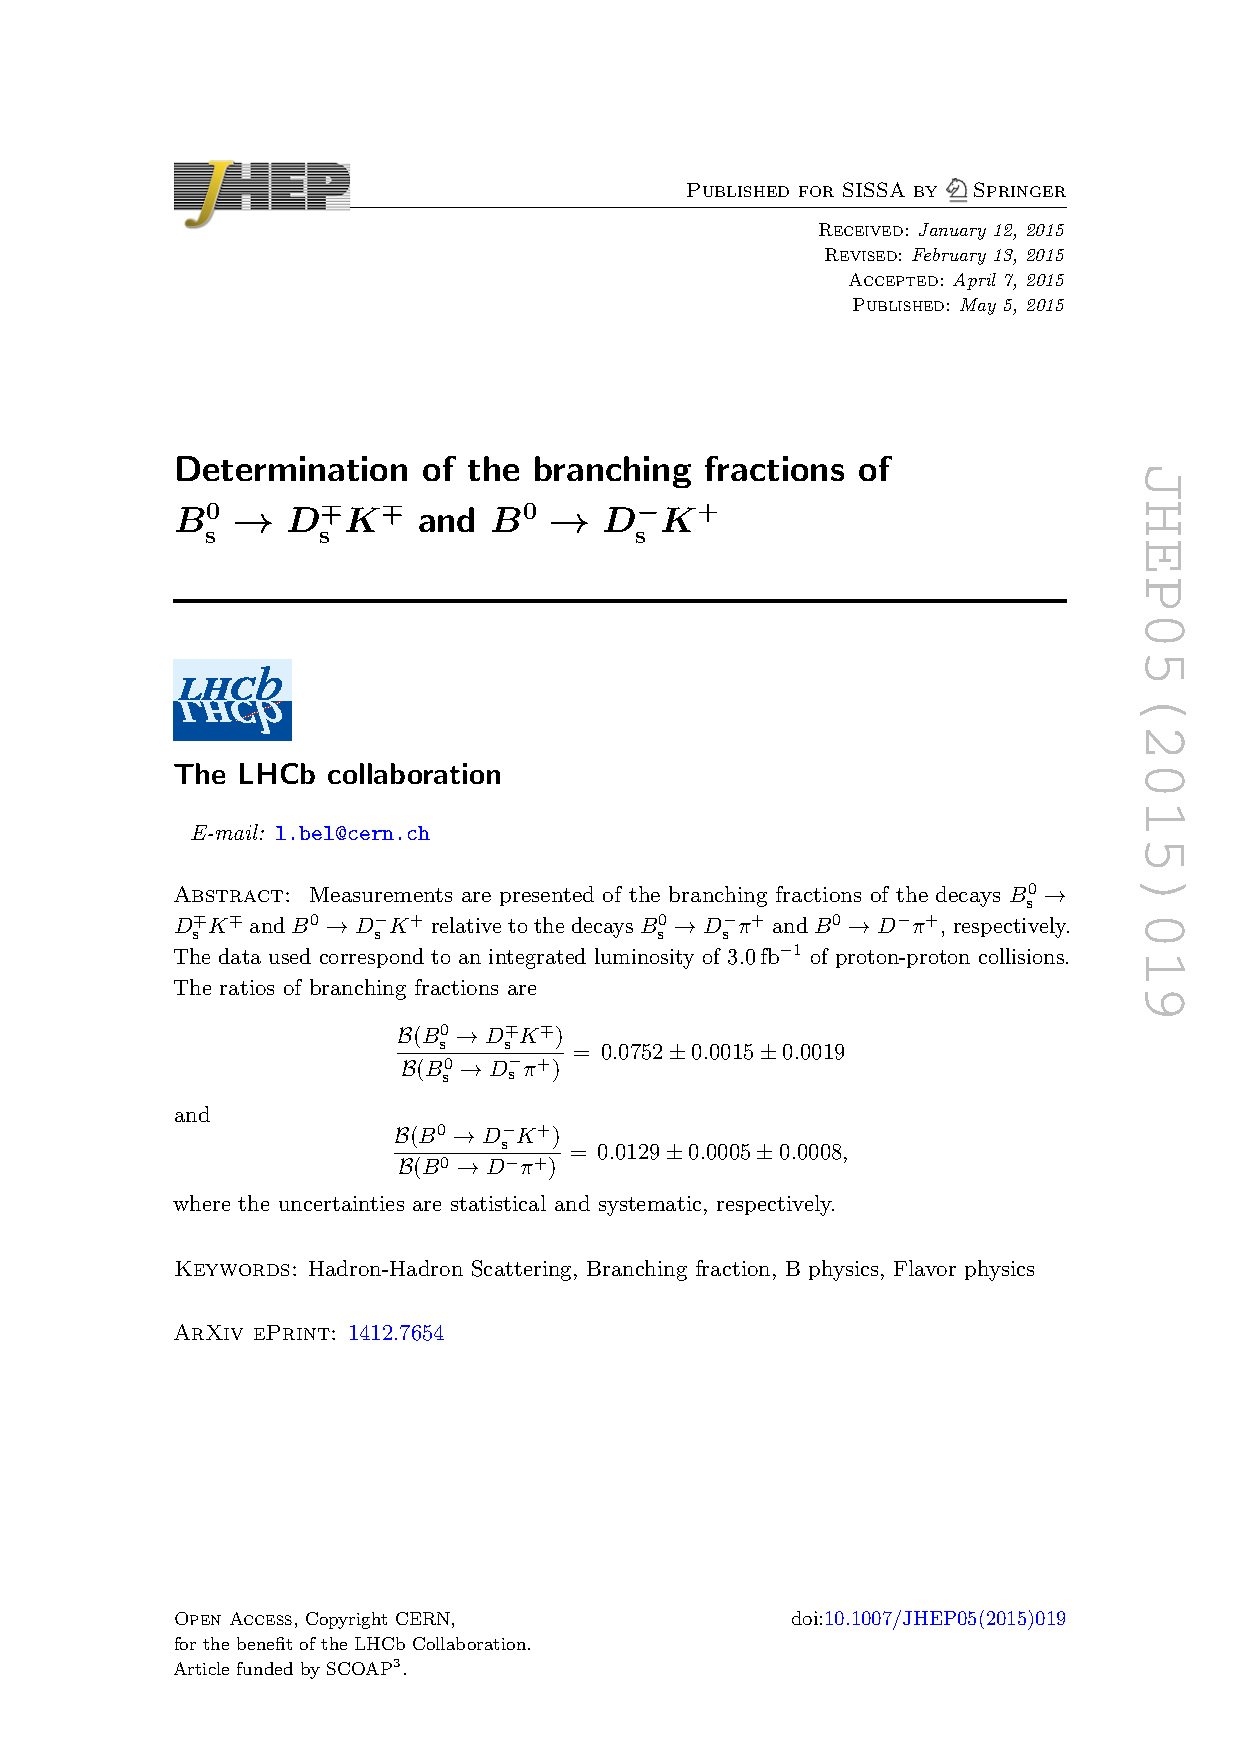
\includepdf[pages=-,scale=1.0,pagecommand={}]{includes/LHCb-PAPER-2014-064.pdf}

